\documentclass[parskip=full]{scrartcl}

\usepackage[utf8]{inputenc}			% Umlaute, Sonderzeichen
\usepackage[ngerman]{babel}			% deutsche Sprache
\usepackage{enumitem}				% Listen
\usepackage{graphicx}				% Grafiken
\usepackage{hyperref}				% Hyperlinks
\usepackage[nonumberlist]{glossaries}		% Glossar
\usepackage{amsmath}
\usepackage{pdfpages}				% PDF einbinden

% Hurenkinder und Schusterjungen verhindern
\clubpenalty10000
\widowpenalty10000
\displaywidowpenalty=10000

\DeclareRobustCommand{\glossfirstformat}[1]{\textit{#1}}	% der erste Verweis im Dokument auf ...
\renewcommand*{\glsdisplayfirst}[4]{\glossfirstformat{#1#4}}	% ... einen Glossarbegriff wird kursiv markiert

% Kriterien sollen nicht kursiv erscheinen
\makeatletter
\renewcommand{\@begintheorem}[2]{\trivlist
	\item[\hskip \labelsep{\bfseries #1\ #2}]}
\makeatother


\makenoidxglossaries

\newglossaryentry{RasPi}{
	name=Raspberry Pi,
	plural=Raspberry Pis,
	description={Der Raspberry Pi ist ein Einplatinencomputer. In diesem Projekt dient der Raspberry Pi als Hardwareplattform, um Messwerte aus angeschlossenen Sensoren auszulesen}
}

\newglossaryentry{PhyPiDAQ}{
	name=PhyPiDAQ,
	description={PhyPiDAQ ist ein Framework zur Erfassung und Analyse von Messwerten mit einem Raspberry Pi. Siehe auch Abschnitt 4.3 ,,PhyPiDAQ`` sowie \url{https://github.com/GuenterQuast/PhyPiDAQ}}
}

\newglossaryentry{Science Labs}{
	name=Science Labs,
	description={Ein Science Lab ist ein Arbeitsplatz, welcher Schülern ermöglicht, wissenschaftliche Forschungen unter kontrollierten Bedingungen durchzuführen} 
}

\newglossaryentry{opensource}{
	name=Open Source,
	description={Software, deren Quelltext öffentlich eingesehen eingesehen werden kann, wird als ,,Open Source`` bzw. ,,quelloffen`` bezeichnet} 
}

\newglossaryentry{osl2}{
	name=OSL\textsuperscript{2},
	description={Open-Source-Lehrsoftware-Labor, siehe \url{https://formal.iti.kit.edu/projects/oslsl/?lang=de}}
}

\newglossaryentry{dragdrop}{
	name=Drag and Drop,
	description={Methode, um mit grafischen Benutzeroberflächen zu interagieren. Dabei wird ein Objekt erst mit der Maus festgehalten und an einen anderen Ort gezogen. Durch das Lösen der Maustaste wird das Objekt platziert}
}

\newglossaryentry{click}{
	name=Click,
	description={Betätigen der linken Maustaste}
}

\newglossaryentry{transformation}{
	name=Transformation,
	plural={Transformationen},
	description={Bausteine vom Typ Transformation haben einen oder mehrere Eingänge sowie einen oder mehrere Ausgänge. Für jeden Ausgang kann  ein Transformationsbaustein eine Vorschrift zur Berechnung eines Ausgangswertes aus einem Satz von Eingangswerten beinhalten. Eine Berechnungsvorschrift soll durch eine mathematische bzw. logische Funktionen oder durch eine programmtechnisch definierte Verarbeitung definiert werden können}
}

\newglossaryentry{konfigdata}{
	name=Konfigurationsdatei,
	plural=Konfigurationsdateien,
	description={Können das Messverhalten anpassen, beispielsweise die Anzahl der Messungen pro Zeiteinheit. Für jeden Sensor gibt es eine eigene Konfigurationsdatei}
}

\newglossaryentry{sensor}{
	name=Sensor,
	plural={Sensoren},
	description={Der Begriff ,,Sensor`` bezeichnet ein technisches Bauteil, welches physikalische Größen misst und analoge oder digitale Messwerte liefert. In unserer Anwendung werden Sensoren abstrakt als grafische Bausteine eines Messkonfiguration präsentiert. Ein solcher (logischer) Sensorbaustein muss alle Informationen referenzieren können, die zum Ansprechen eines tatsächlichen Sensors benötigt werden. Da ein Messgerät Ausgänge bzw. Messkanäle haben kann, muss ein Sensorbaustein mindestens einen oder auch mehrere Ausgänge haben. Eingänge besitzt ein Sensorbaustein nicht}
}

\newglossaryentry{messdaten}{
	name=Messdaten,
	description={Daten, welche die Anwendung von einem Sensor (über PhyPiDAQ-Schnittstelle) oder direkt aus einer Datei erhält}
}

\newglossaryentry{darstellung}{
	name=Darstellung,
	plural={Darstellungen},
	description={Bausteine vom Typ Darstellung haben einen oder mehrere Eingänge. Ein Darstellungsbaustein soll definieren können, wie ein Satz von Eingangswerten die Erstellung bzw. Aktualisierung einer Darstellung beeinflusst. Ausgänge besitzt ein Darstellungsbaustein nicht}
}

\newglossaryentry{python3}{
	name=Python 3,
	description={Python ist eine Skriptsprache, die auf dem Raspberry Pi als Standardsprache zur Programmierung vorgesehen ist. Python wurde zur Implementierung von PhyPiDAQ verwendet}
}

\newglossaryentry{JVM}{
	name={Java Virtual Machine},
	description={Die Java Virtual Machine (JVM) ist eine Plattform für die Ausführung von Java-Software, die von der Firma Oracle für alle gängigen Betriebssysteme bereitgestellt wird}
}

\newglossaryentry{DSGVO}{
	name=DSGVO,
	first={Datenschutz-Grundverordnung (DSGVO)},
	description ={Datenschutz-Grundverordnung der Europäischen Union vom 25. Mai 2018}
}

\newglossaryentry{Musskriterien}{
	name=Musskriterien,
	description ={Werden zusammen mit Soll- und Wunschkriterien bei der Abnahme eines Softwareprodukts überprüft und haben während der Entwicklung höchste Priorität. 
	Dass ein Musskriterium in den nachfolgenden Projektphasen nicht umgesetzt wird, ist nur dann zulässig, falls unerwartet unausweichliche Probleme bei der Umsetzung auftreten. 
	In diesem Fall ist es erforderlich, dass diese Probleme sehr genau dokumentiert werden}
}

\newglossaryentry{Sollkriterien}{
	name=Sollkriterien,
	description ={Werden zusammen mit Muss- und Wunschkriterien bei der Abnahme eines Softwareprodukts überprüft und haben während der Entwicklung mittlere Priorität. 
	Falls ein Sollkriterium umgesetzt werden kann, dann muss es nach Möglichkeit auch realisiert werden. 
	Falls ein Sollkriterium in den nachfolgenden Projektphasen nicht umgesetzt werden kann, so muss dies dokumentiert und begründet werden}
}

\newglossaryentry{Wunschkriterien}{
	name=Wunschkriterien,
	description ={Werden zusammen mit Muss- und Sollkriterien bei der Abnahme eines Softwareprodukts überprüft und haben während der Entwicklung eine niedrige Priorität. 
	Je nach Resourcenlage können sie nach Bearbeitung aller Muss- und Kannkriterien umgesetzt werden. 
	Falls ein Wunschkriterium nicht umgesetzt wird, so muss dies nicht begründet werden}
}

\newglossaryentry{Abgrenzungskriterien}{
	name=Abgrenzungskriterien,
	description ={Abgrenzungskriterien beschreiben Aspekte, die explizit nicht umgesetzt werden sollen.}
}

\newglossaryentry{BenOber}{
	name=Benutzeroberfläche,
	description = {Steht für die Oberfläche, die der Benutzer verwendet um die Anwendung zu bedienen}
}

\newglossaryentry{UI}{
	name=UI,
	description={engl. User Interface; siehe: Benutzeroberfläche}
}

\newglossaryentry{GrafBenOber}{
	name=grafische Benutzeroberfläche,
	description = {Eine Benutzungsschnittstelle, die eine Anwendung durch Fenster, grafische Symbole, Menüs und Mauszeiger bedienbar macht}
}

\newglossaryentry{GUI}{
	name=GUI,
	description={engl. Graphical User Interface; siehe: Grafische Benutzeroberfläche},
}

\newglossaryentry{Konfigurationsbaustein}{
	name=Konfigurationsbaustein,
	plural=Konfigurationsbausteine,
	description ={Teil einer Messkonfiguration, der eine Teilaufgabe bestimmten Typs erfüllen kann. Es gibt Sensorbausteine, Konfigurationsbausteine und Darstellungsbausteine. Liegt am Ausgang eines Bausteins ein Wert an, so kann dieser an den Eingang eines nachgelagerten Bausteins weitergeleitet werden}
}

\newglossaryentry{Benutzerkonfiguration}{
	name =Messkonfiguration,
	plural=Messkonfigurationen,
	description ={Gerichteter zyklenfreier Graph mit Knoten vom Typ Sensor, Transformation oder Darstellung. Hierbei ist zu beachten, dass Sensoren keine Eingangskanten und Darstellungen keine Ausgangskanten haben dürfen}
}

\newglossaryentry{Bausteinprototyp}{
	name=Bausteinprototyp,
	plural=Bausteinprototypen,
	description={Baustein, von dem eine Kopie angelegt wird, wenn der Benutzer ein neues Baustein-Exemplar einem Entwurf hinzufügen möchte}
}

\newglossaryentry{Messlauf}{
	name=Messlauf,
	plural=Messläufe,
	description={Zeitabschnitt, in dem zu definierten Zeitpunkten an allen Bausteinen eines Entwurfs sukzessive die Werte an allen Ausgängen und Eingängen bestimmt werden}
}

\newglossaryentry{Stand-Alone-Kommunikation}{
	name={Stand-Alone-Kommunikation},
	description={Bezeichnet im Kontext unseres Software-Projekt die systeminterne Kommunikation innerhalb eines Betriebssystems, beispielsweise per Inter-Prozess-Kommunikation (IPC)}
	}


\newglossaryentry{Local-Loop}{
	name={Local-Loop},
	description={Bezeichnet einen virtuellen Netzwerkadapter, der Pakete, die durch ihn verschickt werden, unmittelbar danach auch wieder empfängt.}
}

\newglossaryentry{Model-View-Controller}{
	name={Model-View-Controller},
	description={Architekturmuster, dass die Software in die drei Komponenten: Model, View und Controller unterteilt. Dadurch sollen die einzelnen Komponenten unabhängig von einander verändert werden können.}
}

\newglossaryentry{JHotDraw}{
	name={JHotDraw},
	description={JHotDraw ist ein Open-Source, Java-basiertes Framework zur Erstellung von grafischen Editoren. Durch die einfachere Unterstützung von Drag-and-Dop, als komplexere Frameworks eine gute Alternative.}
}

\newglossaryentry{allgemeinen Bausteinprototyp-Informationen}{
	name = {todo},
	description = {todo}
}

\subject{Implementierungsdokumentation}
\title{Definition und Durchführung~von Messwertverarbeitung für~den~Physikunterricht auf~Basis~eines~Raspberry~Pis}
\subtitle{Version 1.0.0}
\author{David Gawron \and Stefan Geretschläger \and Leon Huck \and Jan Küblbeck \and Linus Ruhnke}
\date{\today}


\begin{document}

\maketitle

\clearpage
\tableofcontents 					% generate pdf twice to update

\clearpage
\section{Ziel der Implementierungsdokumentation} \label{einleitung}

\clearpage
\section{Ausarbeitungsstand der Abnahmekriterien} \label{Ausarbeitungsstand}

Im Folgenden werden die Muss-, Soll- und Wunschkriterien aus dem Pflichtenheft herangezogen, das in der ersten Phase des Projekts entstanden ist. Es findet eine Bestandsaufnahme statt, inwieweit die Kriterien erfüllt sind. 

Falls das Softwareprodukt ein Musskriterium nicht wie im Pflichtenheft beschrieben aufweist, so führt dieses Dokument detailliert die Ursachen und Gründe hierfür auf. Falls das Softwareprodukt ein Sollkriterium nicht wie im Pflichtenheft beschrieben aufweist, so beschreibt dieses Dokument zwar nicht in jedem Detail, aber hinreichend informativ die Ursachen und Gründe hierfür. Nicht umgesetzte Wunschkriterien werden lediglich benannt, aber nicht hinterfragt. 

\subsection{Entwurf von Messkonfigurationen}
Es fand ein Fallback statt. Die Messkonfigurationen werden nicht wie gewünscht graphisch durch ein Drag- and Drop Feld erstellt, sondern müssen textuell eingegeben werden. Dadurch verändert sich auch die Betrachtung, wie und ob die folgenden Kriterien überhaupt erfüllt werden können.

\begin{description}
\item{MK 1} Das Musskriterium "`Hinzufügen eines Bausteins aus dem Prototypen-Feld zu der Messkonfiguration"' ist TODO
\item{MK 2} Das Musskriterium "`Anpassen von wichtigen funktionalen Bausteineigenschaften"' ist TODO
\item{MK 3} Das Musskriterium "`Löschen eines Bausteins aus der Messkonfiguration"' ist erfüllt, da der Benutzer die Textuelle Repräsentation eines Bausteins aus der Messkonfiguration entfernen kann.
\item{MK 4} Das Musskriterium "`Erstellen einer Verbindung"' ist umgesetzt. Der Benutzer kann ein Kanaltupel der Liste an Verbindungen hinzufügen und somit eine Verbindung der Messkonfiguration hinzu fügen. 
\item{MK 5} Das Musskriterium "`Löschen einer Verbindung"' ist erfüllt. Der Benutzer kann eine Verbindung aus der Liste der Verbindungen löschen, in dem er das entsprechende Kanaltupel löscht.
\item{SK 1} Das Sollkriterium "`Undo-Redo-Funktion"' ist nicht umgesetzt. Die Messkonfiguration wird textuell erstellt und der Editor unterstützt keine Undo-Redo-Funktion. 
\item{WK 1} Das Wunschkriterium "`Hinzufügen, Bearbeiten und Löschen von ergänzender Informationen zu der Messkonfiguration durch den Benutzer"' ist nicht umgesetzt.
\end{description}
\subsection{Handhabung von Bausteinprototypen}

\begin{description}
	\item{SK 2} Der Benutzer ist in der Lage die Eigenschaften der Bausteinprototypen einzusehen. Jedoch ist die Ansicht auf das Anzeigen der \gls{allgemeinen Bausteinprototyp-Informationen} beschränkt. Der Grund hierfür ist die Anbindung von dem Model an die GUI. Dadurch ist es aktuell nur möglich mit den allgemeinen Bausteinprototyp-Informationen zu arbeiten. Dementsprechend ist das Anzeigen der speziellen Eigenschaften, der Bausteinprototypen, nicht möglich.
	\item{SK 3} Das Kopieren der Bausteinprototypen ist möglich. Auch das Anpassen der allgemeinen Eigenschaften ist möglich. Jedoch können keine generischen Bausteinprototypen erstellt werden. Dafür wäre die Erstellung einer allgemeinen Vorläge nötig gewesen. Diese Erweiterung hätte dem Nutzer jedoch keine weitere Funktionalität geboten. Aus diesem Grund haben wir uns dazu entschieden die Funktion erst in einer eventuellen Erweiterung der Anwendung zu integrieren.
	\item{WK 2} Die Verwendung von erweiternder Software, über eine Schnittstelle, ist nicht mehr vorgesehen. Externe Software kann weiterhin zur Erstellung von Yaml-Dateien genutzt werden. Die so entstandenen Yaml-Dateien können über die Lade-Funktion der Anwendung aufgerufen und anschließend verwendet werden.
	\item{SK 4} Die Anwendung unterscheidet in ihrer jetzigen Form nicht zwischen Benutzerdefinierten- und System-Bausteinen. Deshalb ist es auch hier nur möglich die allgemeinen Eigenschaften der Bausteinprototypen zu ändern.
	\item{SK 5}
\end{description}
		
\subsection{Gewährleisten von Persistenz}

\begin{description}
\item{MK 6} Die verwendeten Bausteine und ihre Anordnung, also die Messkonfiguration, kann in einer Datei gespeichert werden.
\item{MK 7} Messkonfigurationen können aus Dateien geladen werden.
\item{SK 6}
\item{SK 7}
\end{description}

\subsection {Bereitstellung vorgefertigter Teile}

\subsection{Handhabung von Messläufen}

\subsection {Benutzbarkeit der GUI}

\begin{description}
\item[SK 11] Die Funktionalität Aktionen per Drag-and-Drop durchzuführen ist in der aktuellen Version der Anwendung nicht implementiert. Die Gründe hierfür sind die lange Einarbeitungszeit in ein externes Editor-Programm, welches ermöglicht Objekte über Drag-and-Drop zu bewegen. Dies würde das Auswählen eines Editor-Programm beinhalten, die Einarbeitungszeit, die Implemtierung und Integration dieses Programm beinhalten. Durch ein zu spätes Festlegen auf ein Editor-Programm, \gls{JHotDraw} hat die Zeit für die Einarbeitung, Implementierung und Integrierung gefehlt. Deswegen haben wir uns aus Zeitgründen dagegen entschieden ein Editor-Programm zu implementieren. Leider entfällt dadurch eine grundlegende Funktionalität unserer Anwendung, welche bereits fest vorgesehen war und die Benutzung der Anwendung vereinfachen und verbessern würde. Als Weiterentwicklung hat dieses Kriterium eine hohe Priorität.
\item[SK 12] Die Anwendung enthält ein Hilfe-Fenster, welche dem Benutzer eine kurze Beschreibung der Funktionalität der Anwendung und Information über die Anwendung bieten. Die Informationen zu den GUI-Elementen lassen sich jedoch nur aus dem Hilfe Fenster-Text auslesen und nicht interaktiv über Bedienung der GUI-Elemente.
\item[SK 13] Die Anwendung bietet dem Benutzer Information über Fehler-Rückmeldungen über ein Fehlerfenster. 
Vor Fehlverhalten wird nicht gewarnt sondern nur reaktionär auf Fehler reagiert. Die Implementierung des Vorwarnen vor Fehlverhalten hätte sich durch konstante Analyse der Benutzereingaben als zeitintensiv und komplex erwiesen und wurde deswegen nicht umgesetzt.
\item[WK 6] Die Anwendung ist in deutscher Sprache. Das Sprach-Paket lässt sich in der jetzigen Version nicht ändern.
\item[WK 7] Die Festlegung auf ein Konfigurationsfeld, welche eine Konfiguration in schriftlicher Form erstellen lässt führt dazu, dass es keine visuelle Repräsentation von Bausteinen und deren Ein- und Ausgänge gibt.
\item[WK 8] Die Anwendung legt kein festes Farbschema fest und somit ist das Farbschema nicht anpassbar. Die Implementierung ist vorgesehen, aber war zeitlich nicht umsetzbar.
\item[WK 9] Die Anwendung legt eine feste Schriftgröße fest, die sich durch die feste Implementierung der GUI-Tools festlegt und ist somit nicht änderbar. Die Implementierung ist vorgesehen, aber nicht umgesetzt.
\end{description}

\subsection{Abgrenzungskriterien}

\clearpage
\section{Umsetzung des Entwurfs}

Während der Entwurfsphase wurden sowohl UML-Klassendiagramme als auch UML-Sequenzdiagramme erstellt. Zusammen mit der textuellen Beschreibungen der zu erstellenden Software-Elemente bildeten diese die Basis für die Produktion des Quellcodes während der Implementierungsphase. 

In aller Regel lassen sich abstrakte Entwurfsinhalte während der Implementierung nicht in allen Details exakt umsetzen, was verschiedene Gründe haben kann. Bisweilen entpuppt sich auch eine andere Umsetzung als vorteilhafter. Die folgenden Abschnitte halten für jedes Softwaremodul die Abweichungen der Implementierung gegenüber den im Entwurf beschriebenen Strukturen fest. Des Weiteren enthalten sie die Gründe für diese Abweichungen. 
\clearpage

\subsection{Model}

\subsubsection{Ersetzen des Entwurfsmuster Erbauer durch eine Zuständigkeitskette}
Das Paket "`Model.BuildingBlockBuilder"' im Entwurf wurde durch das Paket "`model.block"' ersetzt. Das dort verwendete Entwurfsmuster Erbauer erfüllte nicht die notwendige Anforderung, dass der Benutzter leicht eigene Versionen von Bausteinen in die Anwendung einfügen konnte. Darum wurde der Erbauer durch eine Zuständigkeitskette ersetzt. Hier gibt es keine Methode für jeden Baustein im Director, sondern es gibt nur eine Anzahl von Bearbeitern, die einen Block eines Types erstellen. Wenn also der Benutzter eine eigene Transformation erstellen will, kann er die .yaml Datei einer bereits vorhandenen Transformation kopieren und einige Parameter (außer Typ und subtyp) verändern. Die resultierende Transformation wird dann von der Anwendung als eine erkannt und kann dann auch dort verwendet werden.
Dadurch entfallen alle folgenden Klassen des Entwurfs:

\begin{description}
\item{} Builder
\item{} TransformationBuilder
\item{} RepresentationBuilder
\item{} XYRepresentationBuilder
\item{} TableRepresentationBuilder
\item{} SensorBuilder
\item{} VirtualSensorBuilder
\item{} PhysicalSensorBuilder
\item{} SnakeYamlParser
\item{} java.util.hashmap
\end{description}

sowie all diese öffentlichen Methoden in der Director Klasse:

\begin{description}
\item{} createSensorFromYaml
\item{} constructTransformation
\item{} constructXYRepresentation
\item{} constructNTimeRepresentation
\item{} constructDS18B20TemperatureSensor
\item{} constructBMPx80PressureSensor
\item{} constructINA219CurrentAndVoltageSensor
\item{} constructMMA8451Accelerometer
\item{} constructTransformation

\end{description}

Statt dessen wurden folgende Klassen hinzugefügt:
\begin{description}
\item{} GeneralBlockKvProcessor
\item{} KvProcessor
\item{} SensorKvProcessor
\item{} PhysicalSensorKvProcessor
\item{} VirtualSensorKvProcessor
\item{} RepresentationKvProcessor
\item{} TableRepresentationKvProcessor
\item{} XYRepresentationKvProcessor
\item{} TransformationKvProcessor
\end{description}

und die Methode constructBuildingBlock zum Director und zu jedem Bearbeitern die Methode processKvPair hinzugefügt. Dabei unterscheiden sich die Methoden der einzelnen Bearbeitern zwar nicht im Namen, aber in ihrer Funktion. Jeder Bearbeiter leitet entweder die Anfrage weiter oder erstellt einen Blocktyp und gibt ihn zurück. 

\subsection{GUI}

\subsection{Controller}

\subsection{Backend}

\subsection{Cache}

\subsection{File-Service}

\section{Realer Implementierungsablauf}

Dieser Abschnitt führt auf, inwieweit der tatsächliche zeitliche Implementierungsablauf vom geplanten Ablauf abgewichen ist, und beschreibt die Ursachen und Gründe für diese Abweichungen. Abhängigkeiten zwischen den Implementierungsschritten und kritische Pfade stehen hierbei besonders im Fokus.

Von Abweichungen betroffene Softwareelemente werden nicht im Einzelnen aufgeführt, sondern es werden lediglich in Bezug auf die Abweichungsgründe die Gruppen der betroffenen Softwareelemente benannt.

\section{Anhang}

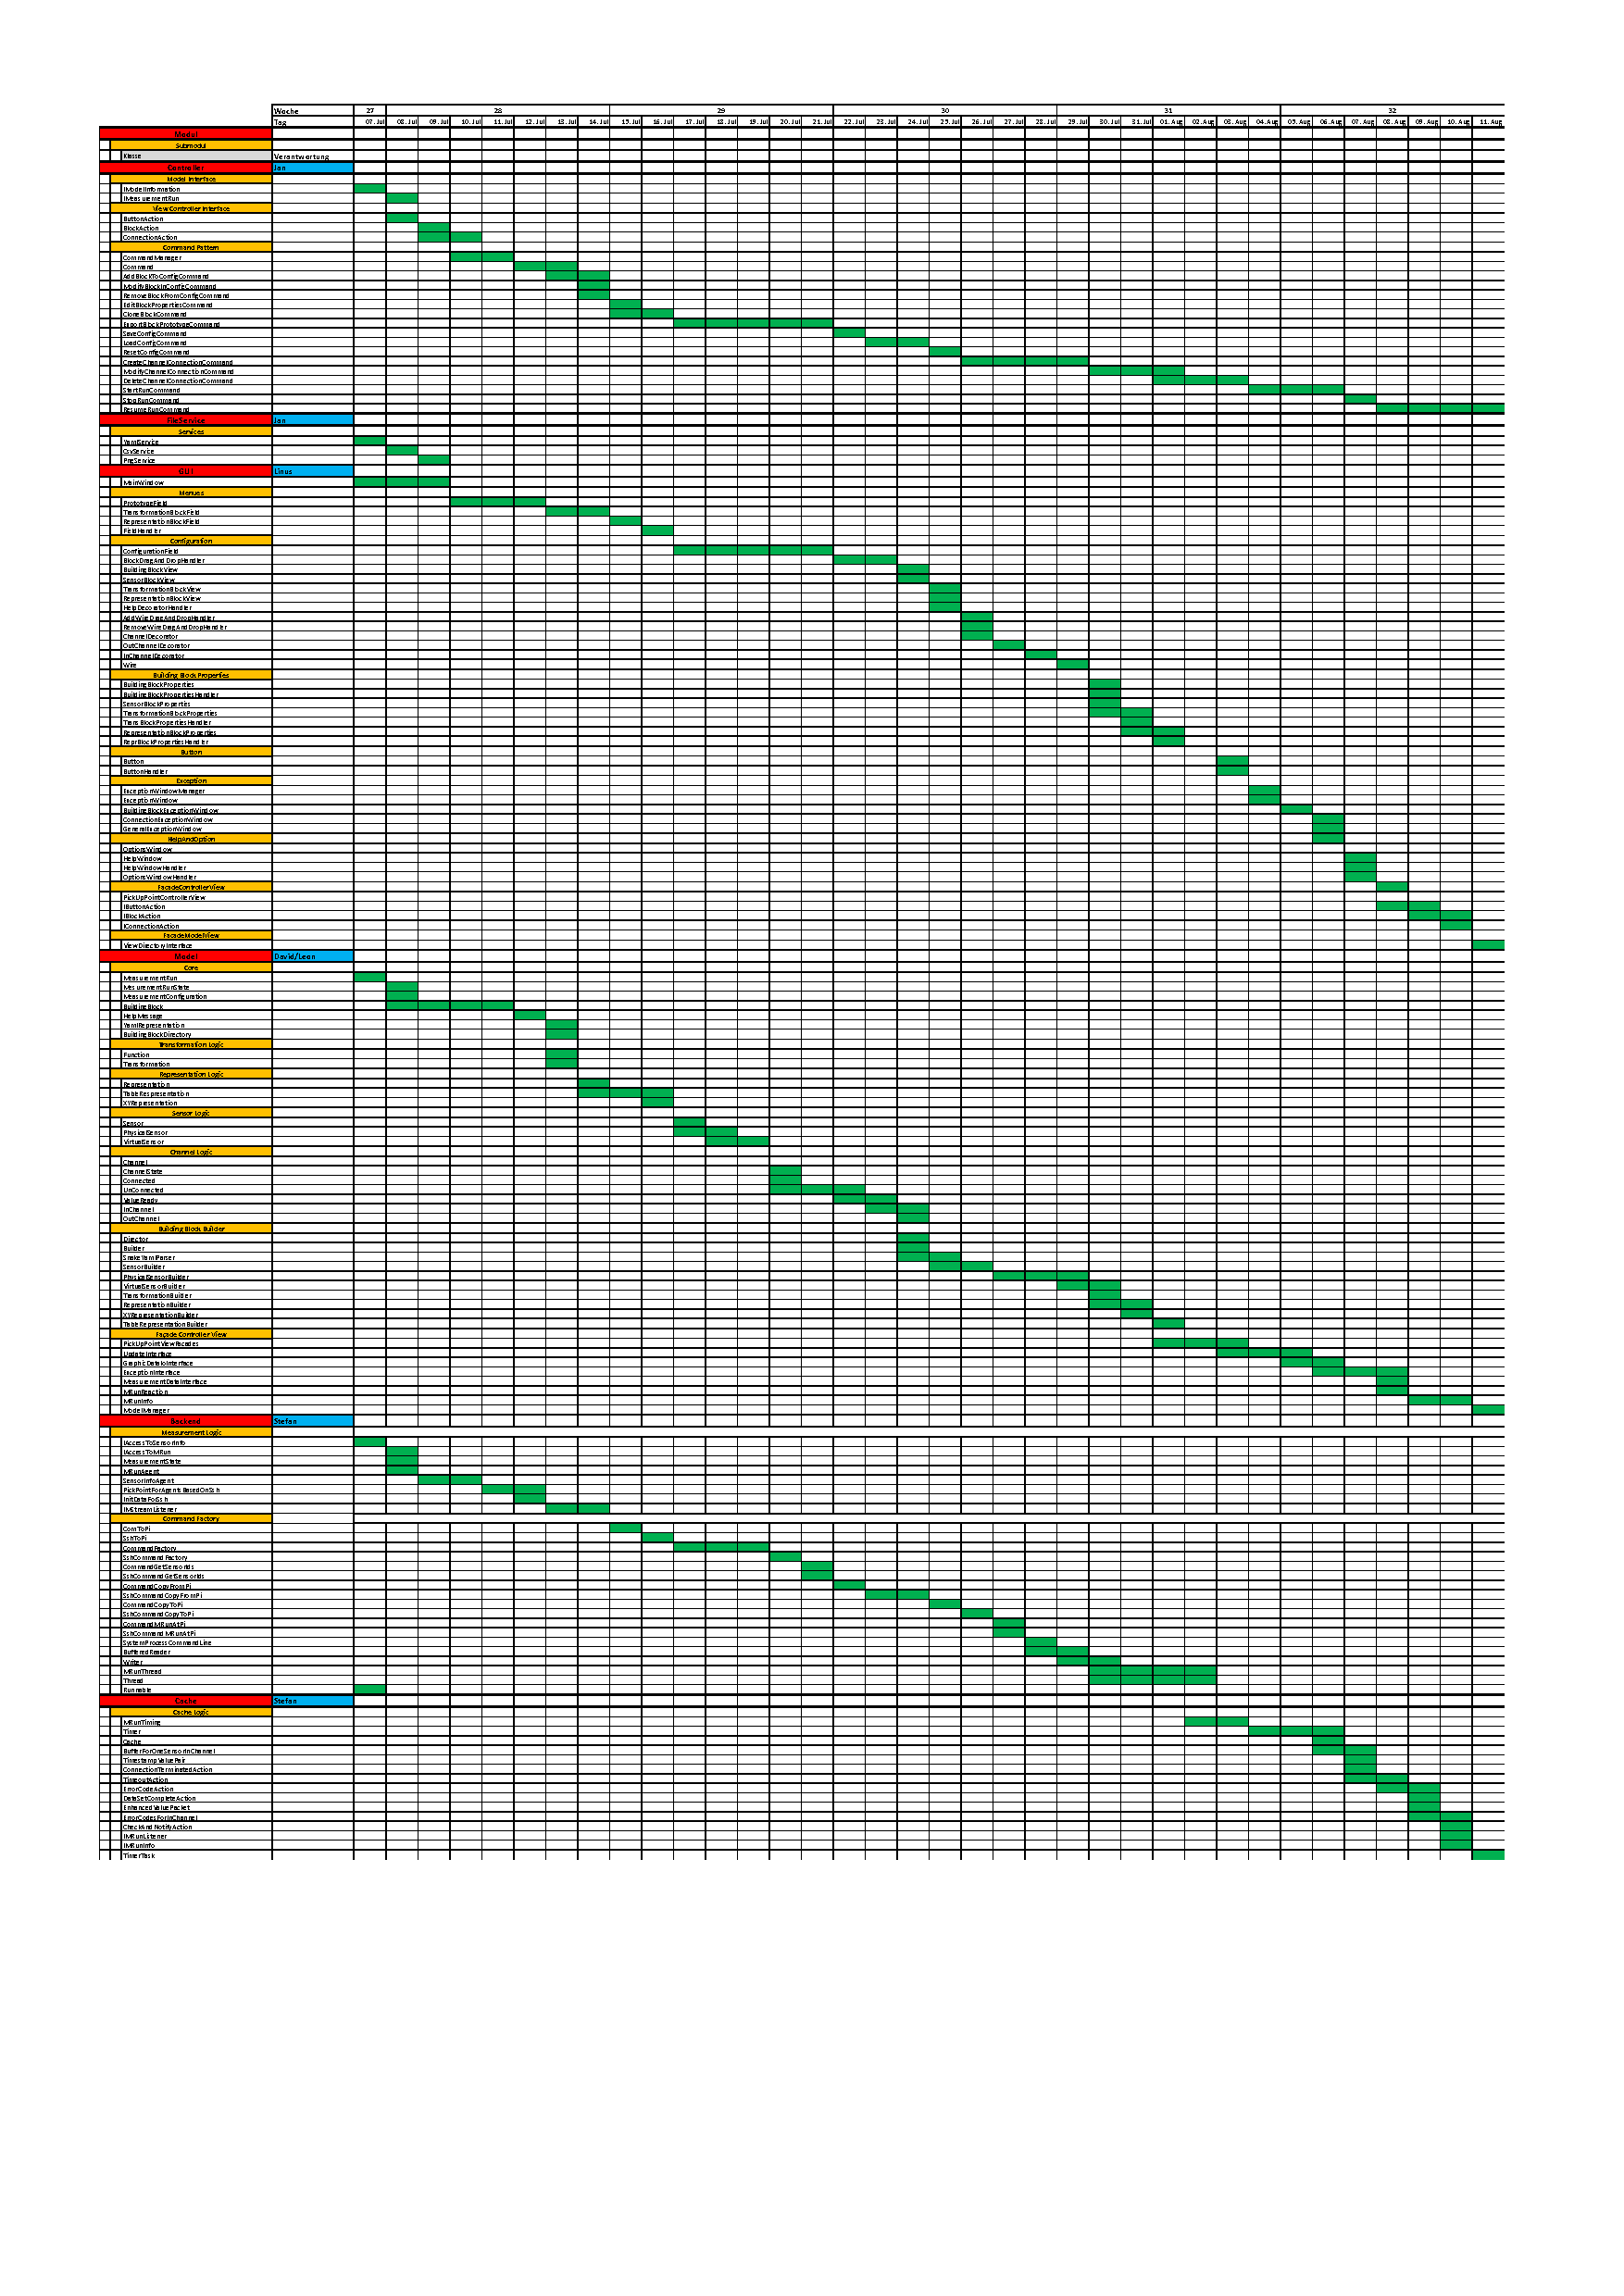
\includepdf{Grafiken/Implementierungsplan.pdf}

\clearpage
\section{Glossar}\label{glossar}

\renewcommand*{\glossarysection}[2][]{}	% prevents double glossary section heading
\printnoidxglossaries				% generate pdf twice when adding new entries

\end{document}\grid
